\documentclass[12pt]{article}
\usepackage{float}
\restylefloat{table}
\usepackage{graphicx}
\usepackage{rotating}
\usepackage{color}
\usepackage[dvipsnames]{xcolor}
\usepackage{enumitem}
\usepackage{sidecap}
\usepackage[top=15mm, bottom=15mm, left=15mm, right=15mm]{geometry}
\usepackage{multicol}
\usepackage[dvipsnames]{xcolor}
\usepackage{wrapfig}
\usepackage{hyperref}
\usepackage{courier}

\fboxrule=2pt%border thickness

\pagenumbering{gobble}

\setlength\parindent{0pt}

\begin{document}
\title{DEVILS - Support Astronomer Guide}
\begin{center}

\begin{figure}
\begin{center}
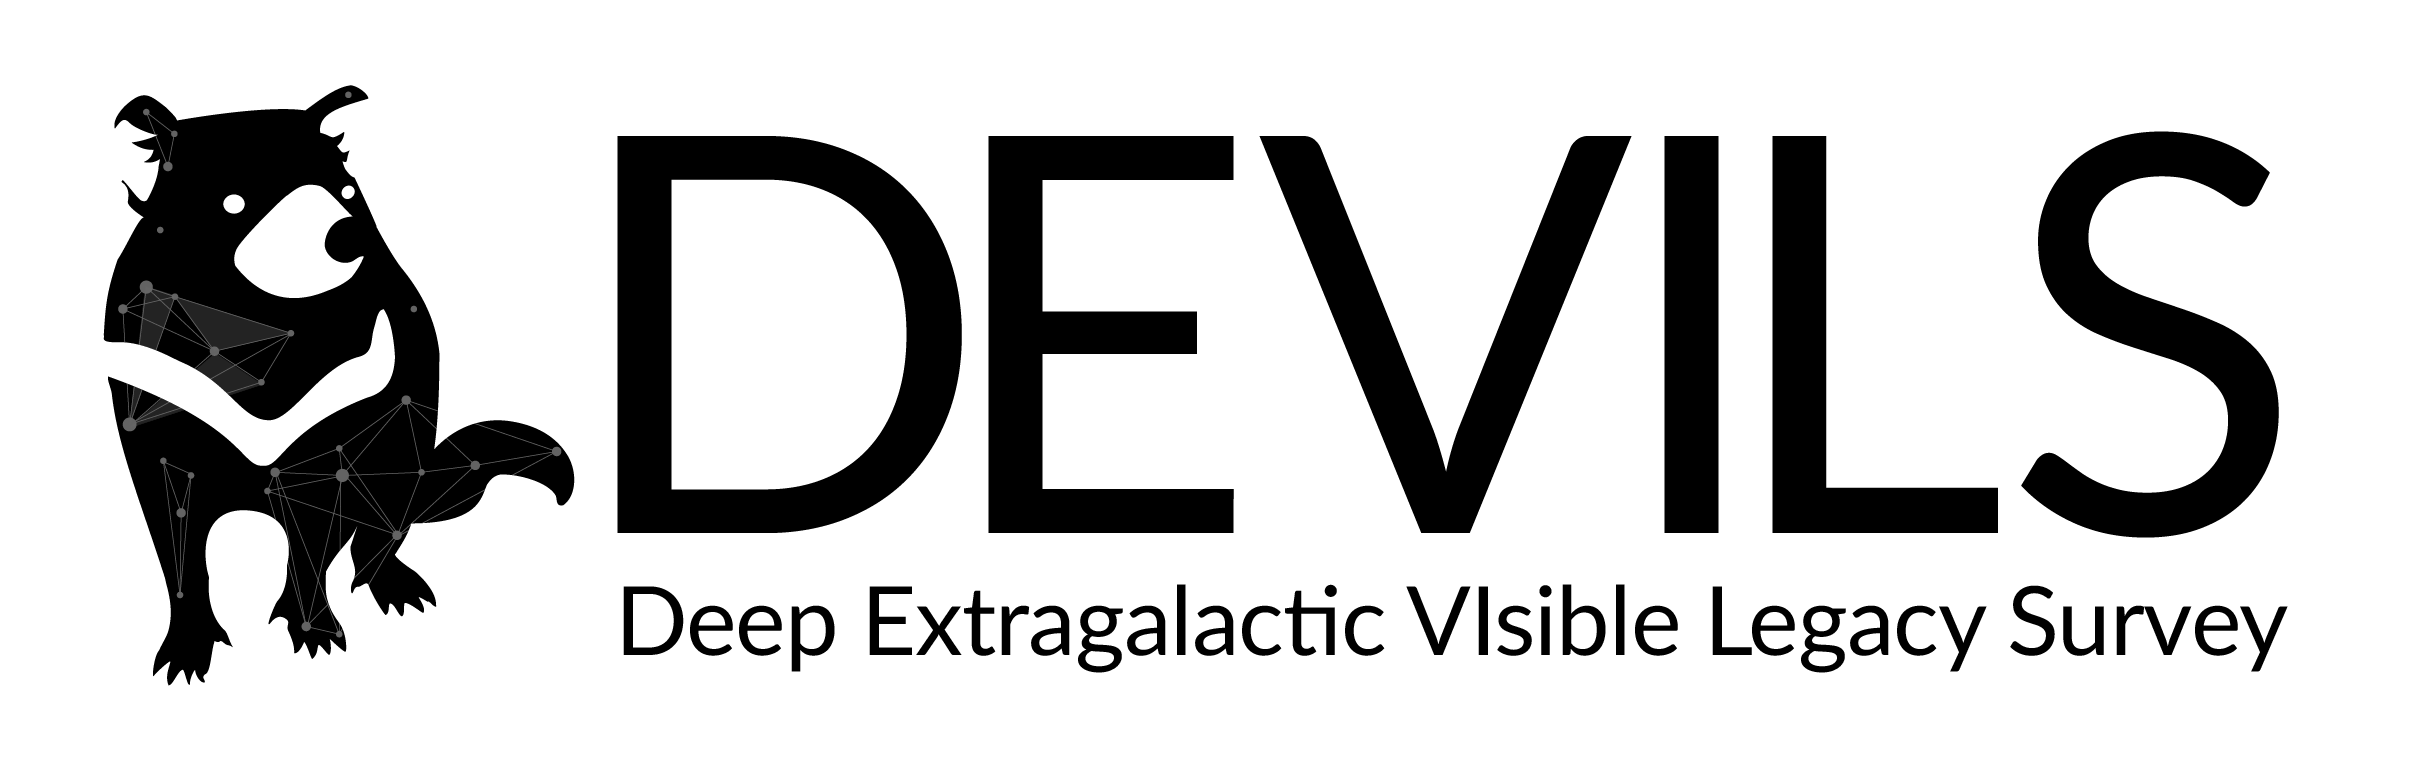
\includegraphics[scale=0.8]{devils-logo_big.png}
\end{center}
\end{figure}

\Huge {\textcolor{PineGreen}{\textbf{Support Astronomer Guide}}}
\Huge {\textcolor{PineGreen}{\textbf{ Version 0.1}}}\\
\Large \textbf{Luke Davies (21/12/2017)}\\
\end{center}
\normalsize

\section{Overview}

\section{In The Day}

\subsection{Initial Checks}

\begin{enumerate}

\item \textbf{Check the run number is set to 1.} This should be done in a pop-up window that appears each day at 11am.

\item \textbf{Check/Set program ID to correct value}. This is done in the \textsf{{\textcolor{purple}{2df Control Task}}} $>$ Commands window ({\textcolor{orange}{ORANGE 1}}  in Figure \ref{fig:Control}).  

\item \textbf{Set ADC to NULL}. This is also done in the \textsf{{\textcolor{purple}{2df Control Task}}} window. Select `more' under ADC ({\textcolor{red}{RED 1}} in Figure \ref{fig:Control}), and the `null ADC'.

\item \textbf{Check configuration files are available}. Check that the configuration files for the night have been copped to the correct \textbf{/configs/devils/YYMMDD/} directory on \texttt{aatlxh}.

\end{enumerate}


\begin{figure}
\begin{center}
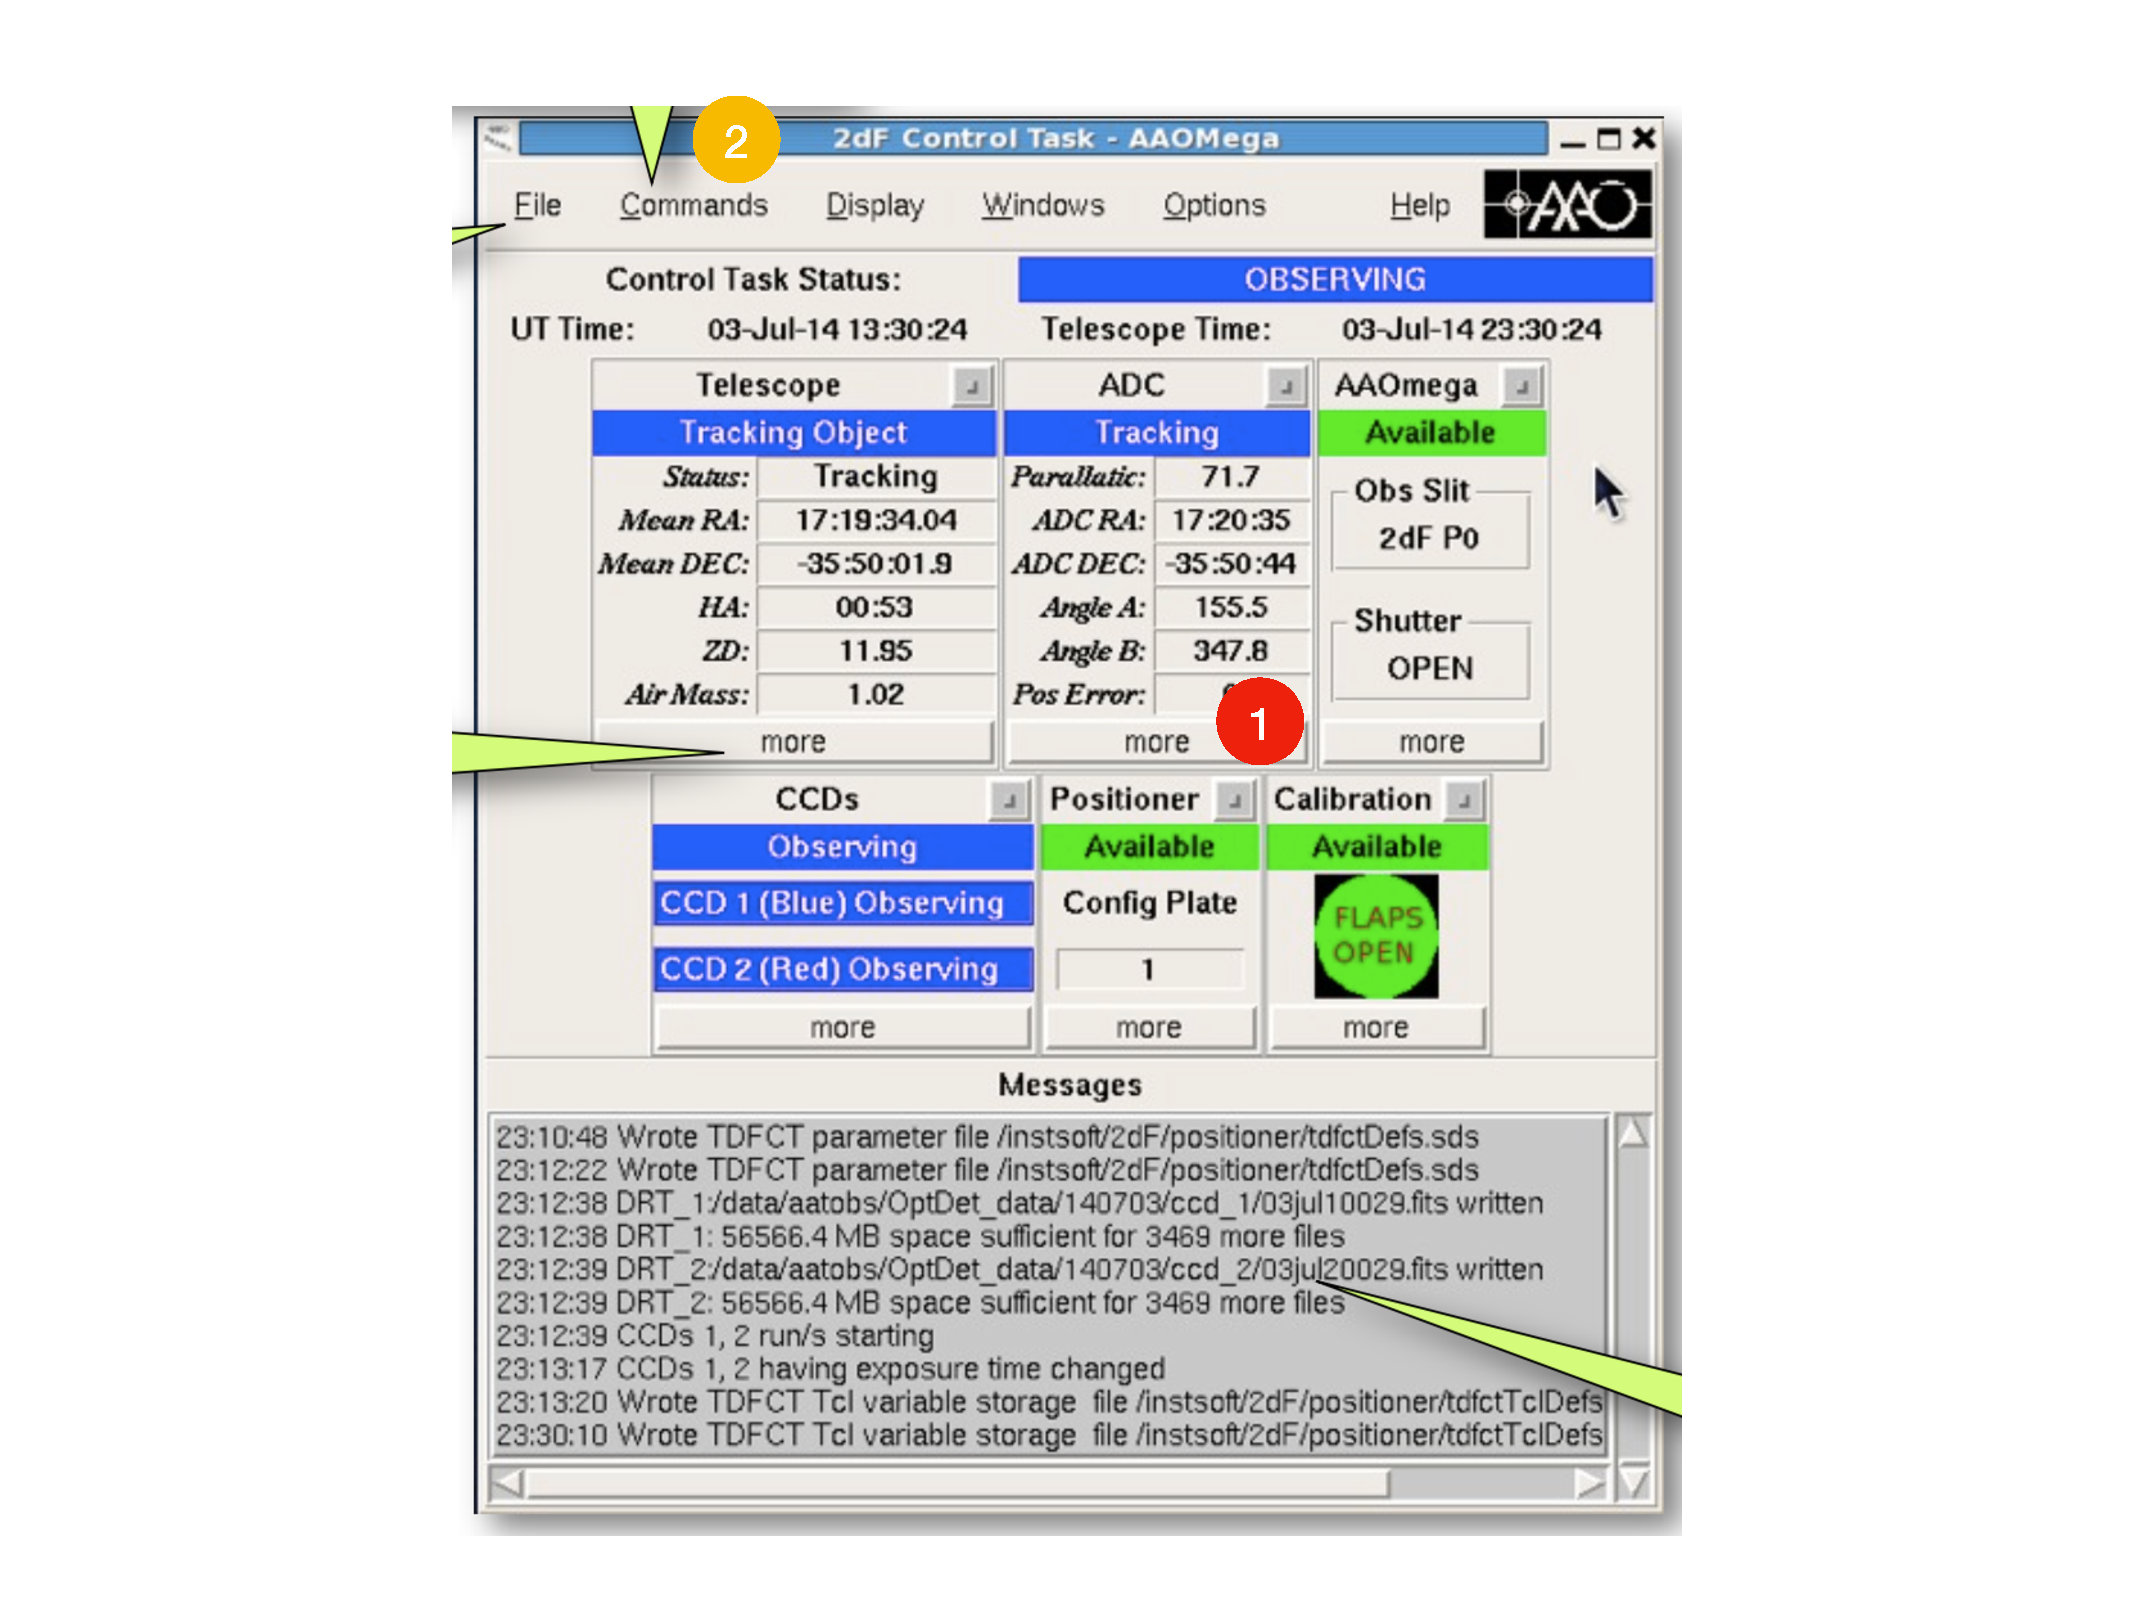
\includegraphics[scale=0.8]{2DFControlTaskWindow.pdf}
\caption{2dF Control Task Window}
\label{fig:Control}
\end{center}
\end{figure}

\subsection{Take Biases}

\vspace{5mm}


{\large \textsf{Use the {\textcolor{purple}{CCD Control}} window.}}

\begin{enumerate}

\item \textbf{Ensure dark screens are closed on AAOmega}. This needs to be done in the spectrograph room. Drop the screen over both the red and blue CCD.

\item \textbf{Set exposure time to 0}. This is set in the box labelled with the {\textcolor{red}{RED 1}} in Figure \ref{fig:CCD}.

\item \textbf{Set observation to `Bias'}. Found at {\textcolor{red}{RED 2}} in Figure \ref{fig:CCD}.

\item \textbf{Set run type to `Normal'}. Found at {\textcolor{red}{RED 3}} in Figure \ref{fig:CCD}.

\item \textbf{Set exposures to 10}. Exposure numbers are set at the {\textcolor{red}{RED 4}} in Figure \ref{fig:CCD}.

\item \textbf{Start running exposures}. This is done by hitting the `Start CCD Run' button - {\textcolor{blue}{BLUE 7}} in Figure \ref{fig:CCD}.While the exposures are 0sec, this will take $\sim15$min as the CCDs. 

\item \textbf{Lift dark screen}. Once finished, ensure that the dark screens are lifted.

\end{enumerate}

\begin{figure}
\begin{center}
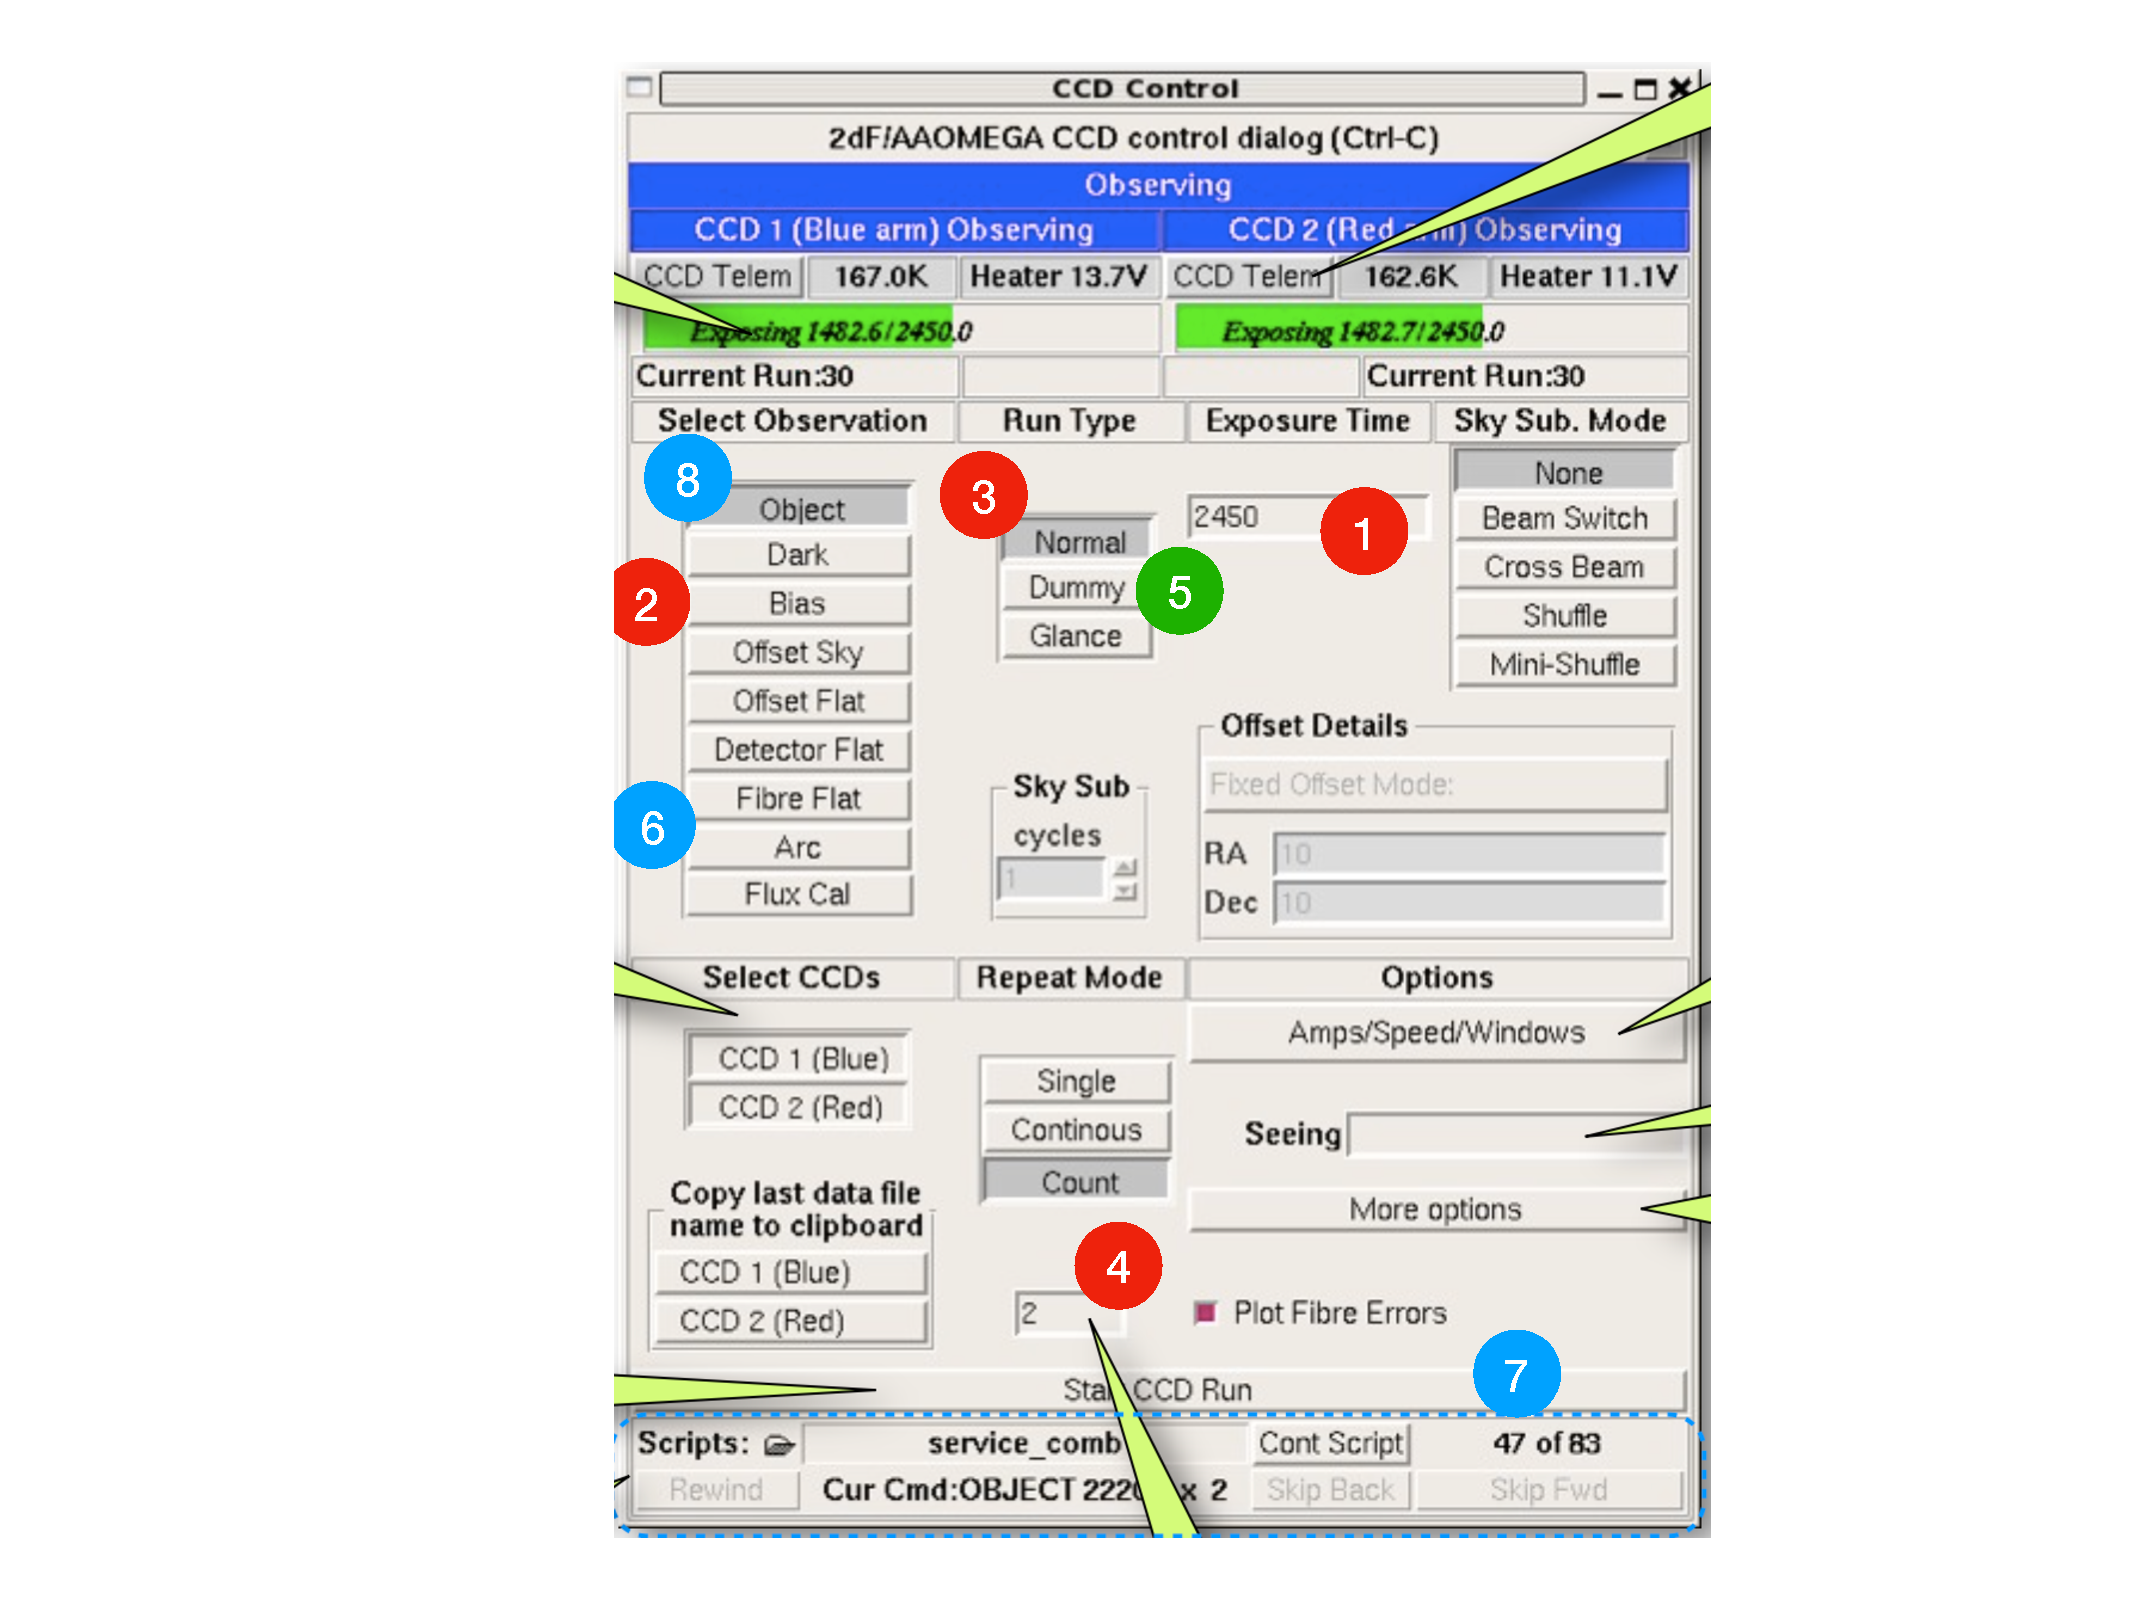
\includegraphics[scale=0.8]{CCDControlWindow.pdf}
\caption{CCD Control Window}
\label{fig:CCD}
\end{center}
\end{figure}

\subsection{Configure First Plate on 2dF}

\vspace{5mm}


{\large \textsf{Use the {\textcolor{purple}{Positioner Control}} window.}}

\begin{enumerate}

\item \textbf{Check Plate Number}. Check that the correct plate number (0,1) is the configuration plate currently on 2dF. This can be found in the \textsc{\textcolor{purple}{Positioner Control}} window ({\textcolor{red}{RED 1}} in Figure \ref{fig:Pos}, or at the top of the \textsc{\textcolor{purple}{Positioner}} window ({\textcolor{red}{RED 2}} in Figure \ref{fig:Pos}). You should also see that it is the top plate in the small image on the  \textsc{\textcolor{purple}{Positioner}} window ({\textcolor{red}{RED 3}}). 

\item \textbf{If needed, Tumble}.  If you need to change the plate you can do so in the \textsc{\textcolor{purple}{Positioner Control}} window but hitting 'Tumble' at the {\textcolor{orange}{ORNAGE 5}}.

\item \textbf{Copy .sds file for configuration}. In the xterm copy the configuration file you want to use from \textbf{/configs/devils/YYMMDD/} to \textbf{instsoft/2df/configs/*mon*17/*DDmon*/}.

\item \textbf{Load .sds file for configuration}. You can now see the configuration file to load. Select `Find File' in the \textsc{\textcolor{purple}{Positioner}} window ({\textcolor{green}{GREEN 6}} in Figure \ref{fig:Pos}).

\item \textbf{Set the start time and duration}. For your configuration, set the start time (local time in 24h format, {\textcolor{purple}{PURPLE 7}}) and duration  (in hours, {\textcolor{purple}{PURPLE 8}}) in Figure \ref{fig:Pos}.

\item \textbf{Set the Weather Conditions}. Select the `Weather' tab in the \textsc{\textcolor{purple}{Positioner Control}} window. The hit `Fetch from Weather...' button. NOTE: if you are configuring in the day, take a few degrees off the fetched weather for the drop in the night. Write down the `Positioning Stats" on the 2dF observer sheet. 

\item \textbf{Check Wavelengths}. Select the `Wavelengths' tab in the \textsc{\textcolor{purple}{Positioner Control}} window. Check that they are 6000, 2000, 5000.

\item \textbf{Check Input Parameters}. Return to the correct plate tab on the \textsc{\textcolor{purple}{Positioner Control}} window and check the Field, Plate, Time, Duration and configuration you have set.   

\item \textbf{Check Input Parameters}. Return

\end{enumerate}

\end{document}

